\documentclass[11pt]{article}
\usepackage{../EllioStyle}
\usepackage{fancyvrb}
\usepackage{pdfpages}
\usepackage{xcolor}

\title{Midterm}
\author{Elliott Pryor}
\date{29 Sept 2020}


\begin{document}
\maketitle

\begin{huge}
\textit{*Note: Problems are out of order to remove large blank spaces. Problem ordering is 2, 1, 3}
\end{huge}

\problem{2}

\begin{Verbatim}
// In UML book 5.1.2.1 it gives example 5-3 of code for an Association Class
// So this is copied from the book

public class Account {
    private String name;
    private Category[] categories;
    private DiaryEntry[] entries;
}


public class Category {
    private String name;
}

public class DiaryEntry {
    private String name;
    private Category[] categories;
}
\end{Verbatim}

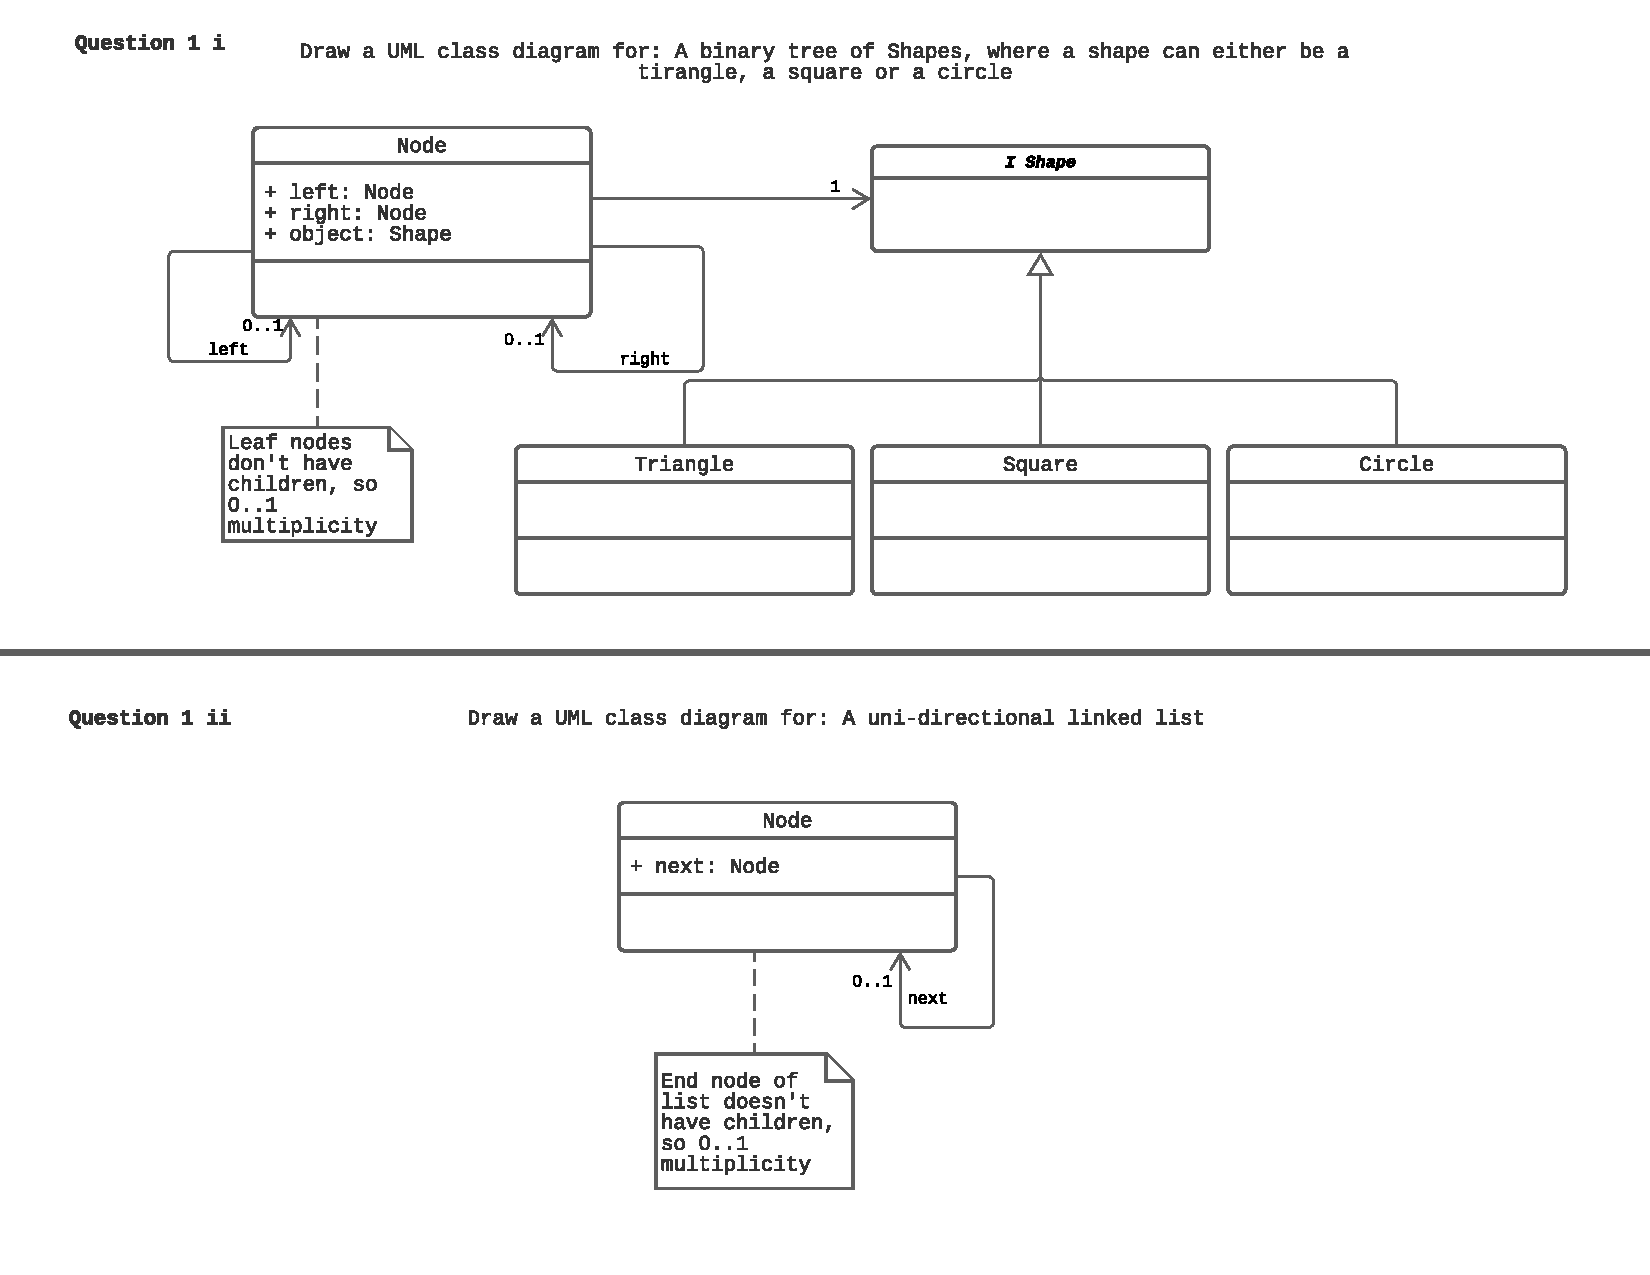
\includepdf[pages={1}]{./Exam1_LucidChart.pdf}



\problem{3}

\begin{figure}[H]
    \centering
    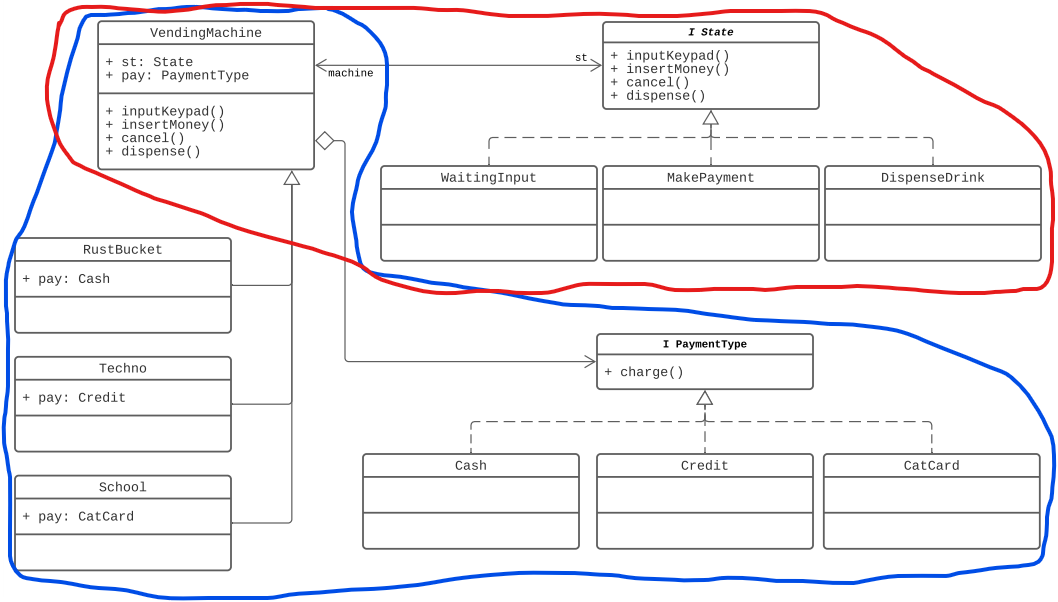
\includegraphics[scale=0.5]{./coupled_q3.png}
    \caption{Coupled components are circled}
    \label{fig:circled}
\end{figure}

In figure \ref{fig:circled}, the coupled components are circled. \textcolor{red}{The components circled in red are the state pattern}, and \textcolor{blue}{the components circled in blue are the strategy pattern}. This depicts a vending machine. There are multiple states the vending machine could be in (similar to the gumball machine from class). Each vending machine can use a different payment type (strategy pattern) that could be swapped out. So if money is inserted in the makePayment state it will use the pay object (type PaymentType) to collect money in a variety of ways. This combines the strategy pattern (changeable PaymentType) and the State pattern (different VendingMachine states). 

\includepdf[pages={2}]{./Exam1_LucidChart.pdf}



\end{document}